\documentclass[10pt,compress,usetitleprogressbar,mathserif]{beamer}
\usepackage[spanish, es-tabla,es-noquoting,es-noshorthands]{babel}
\usepackage{etex}
\usepackage{tikz} % Tikz (para el tema)
\usepackage{showexpl} % ???
\usepackage{amsthm}  %%
\usepackage{amsmath} % Matemáticas
\usepackage{amssymb} %%
\usepackage{graphicx} % Imágenes

\usepackage{listings} % Códigos

\definecolor{backg}{HTML}{F2F2F2}    % Fondo
\definecolor{comments}{HTML}{BDBDBD} % Comentarios
\definecolor{keywords}{HTML}{08388c} % Palabras clave
\definecolor{strings}{HTML}{0489B1}  % Strings

\lstset{
%language=,
basicstyle=\ttfamily\small,
breaklines=true,
backgroundcolor=\color{backg},
keywordstyle=\color{keywords},
commentstyle=\color{comments},
stringstyle=\color{strings},
tabsize=2,
% Acentos, ñ, ¿, ¡ (tex.stackexchange.com/questions/24528)
extendedchars=true,
literate={á}{{\'a}}1 {é}{{\'e}}1 {í}{{\'i}}1 {ó}{{\'o}}1
         {ú}{{\'u}}1 {ñ}{{\~n}}1 {¡}{{\textexclamdown}}1
}

\lstdefinelanguage{JavaScript}{
  keywords={typeof, new, true, false, catch, function, return, null, catch, switch, var, if, in, while, do, else, case, break},
  keywordstyle=\color{blue}\bfseries,
  ndkeywords={class, export, boolean, throw, implements, import, this},
  ndkeywordstyle=\color{darkgray}\bfseries,
  identifierstyle=\color{black},
  sensitive=false,
  comment=[l]{//},
  morecomment=[s]{/*}{*/},
  commentstyle=\color{purple}\ttfamily,
  stringstyle=\color{red}\ttfamily,
  morestring=[b]',
  morestring=[b]"
}

% Solarized palette
\definecolor{solarizedBase03}{HTML}{002B36}
\definecolor{solarizedBase02}{HTML}{073642}
\definecolor{solarizedBase01}{HTML}{586e75}
\definecolor{solarizedBase00}{HTML}{657b83}
\definecolor{solarizedBase0}{HTML}{839496}
\definecolor{solarizedBase1}{HTML}{93a1a1}
\definecolor{solarizedBase2}{HTML}{EEE8D5}
\definecolor{solarizedBase3}{HTML}{FDF6E3}
\definecolor{solarizedYellow}{HTML}{B58900}
\definecolor{solarizedOrange}{HTML}{CB4B16}
\definecolor{solarizedRed}{HTML}{DC322F}
\definecolor{solarizedMagenta}{HTML}{D33682}
\definecolor{solarizedViolet}{HTML}{6C71C4}
\definecolor{solarizedBlue}{HTML}{268BD2}
\definecolor{solarizedCyan}{HTML}{2AA198}
\definecolor{solarizedGreen}{HTML}{859900}

\usetheme{epstfg}
\setbeamertemplate{note page}[compress]
\setbeamertemplate{itemize subitem}{\tiny\raise1.5pt\hbox{\donotcoloroutermaths$\blacktriangleright$}}
\title{HTTP Live Streaming}
\author{Pablo Baeyens \and José Manuel Muñoz}
\date{Fundamentos de Redes}
\def\inline{\lstinline[basicstyle=\ttfamily]}

\begin{document}
\maketitle

\begin{frame}{Índice}
  \tableofcontents
\end{frame}

\begin{frame}{¿Qué es HLS?}
  HTTP Live Streaming es un protocolo de transmisión de \textbf{streaming} y \textbf{vídeo bajo demanda}.

  Es soportado por dispositivos móviles con iOS y Android y ha sido utilizado por páginas como TED, Twitter o Twitch
\end{frame}

\begin{frame}{Características}
  Sus principales características son:
  \begin{itemize}
    \item Se transmite mediante \textbf{HTTP} % no necesita más configuración
    \item Permite adaptar la calidad del vídeo según la conexión
    \item Permite encriptar el vídeo y transmitir metadatos adicionales
    \item Puede utilizarse en la mayor parte de dispositivos
  \end{itemize}
\end{frame}

\begin{frame}{Visión general}
  \only<1>{
  \begin{itemize}
    \item El vídeo se divide en segmentos en distintas calidades
    \item Se crea una archivo índice con los segmentos
    \item Se transmite al cliente mediante HTTP
    \item Se reconstruye en el cliente
  \end{itemize}
  }
  \only<2>{
  \begin{center}
    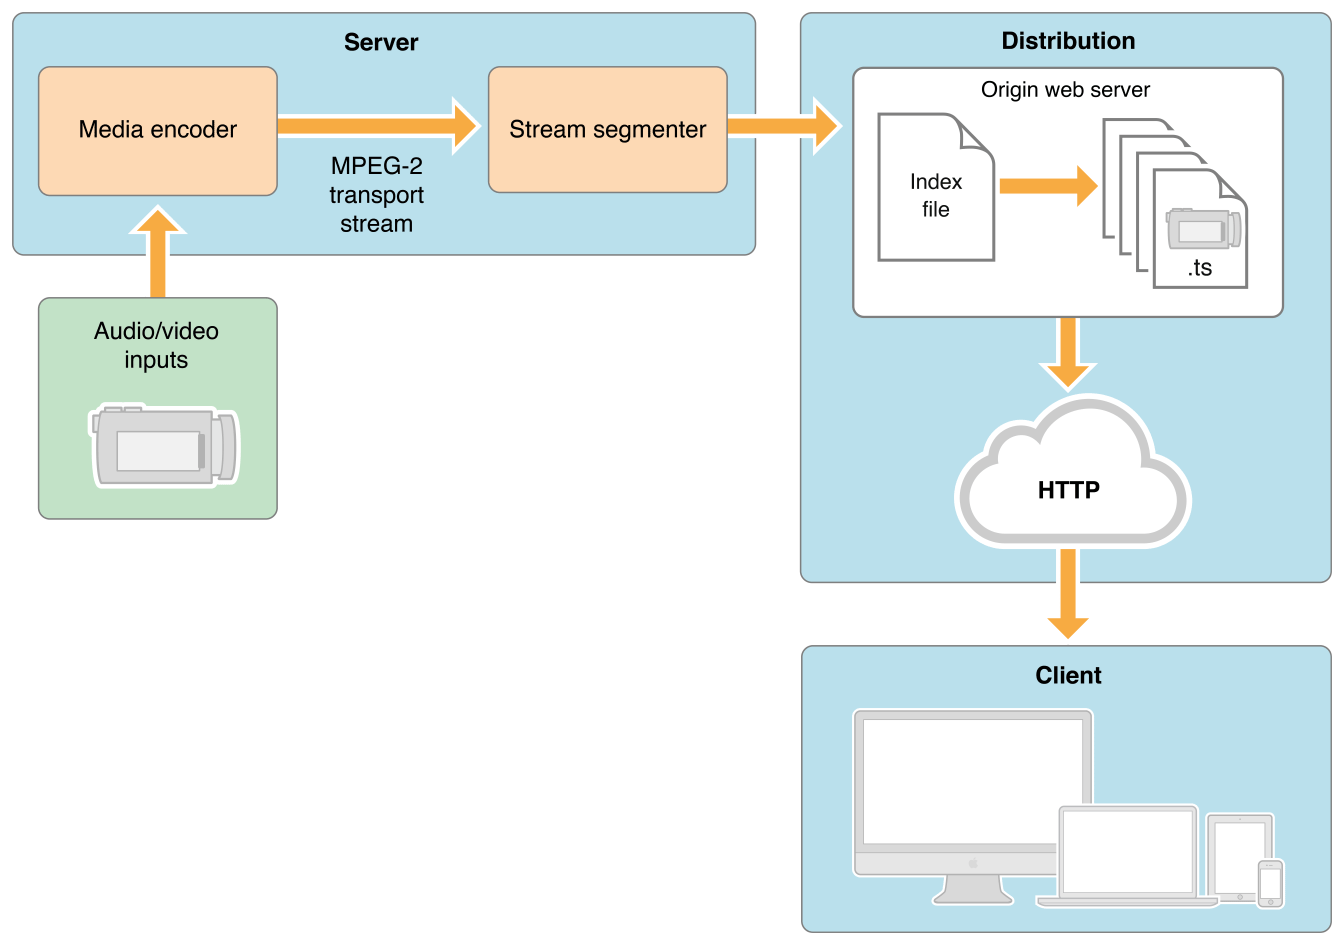
\includegraphics[scale=0.2]{img/visionGeneral.png}
  \end{center}}
\end{frame}


\begin{frame}{Tipos de sesión}
  Los vídeos transmitidos pueden ser:
  \begin{itemize}
    \item En \textbf{tiempo real} (no permite avance y retroceso en general)
    \item Como \textbf{vídeo bajo demanda} (permite avance y retroceso)
  \end{itemize}
\end{frame}

\begin{frame}{Codificación y segmentación}
  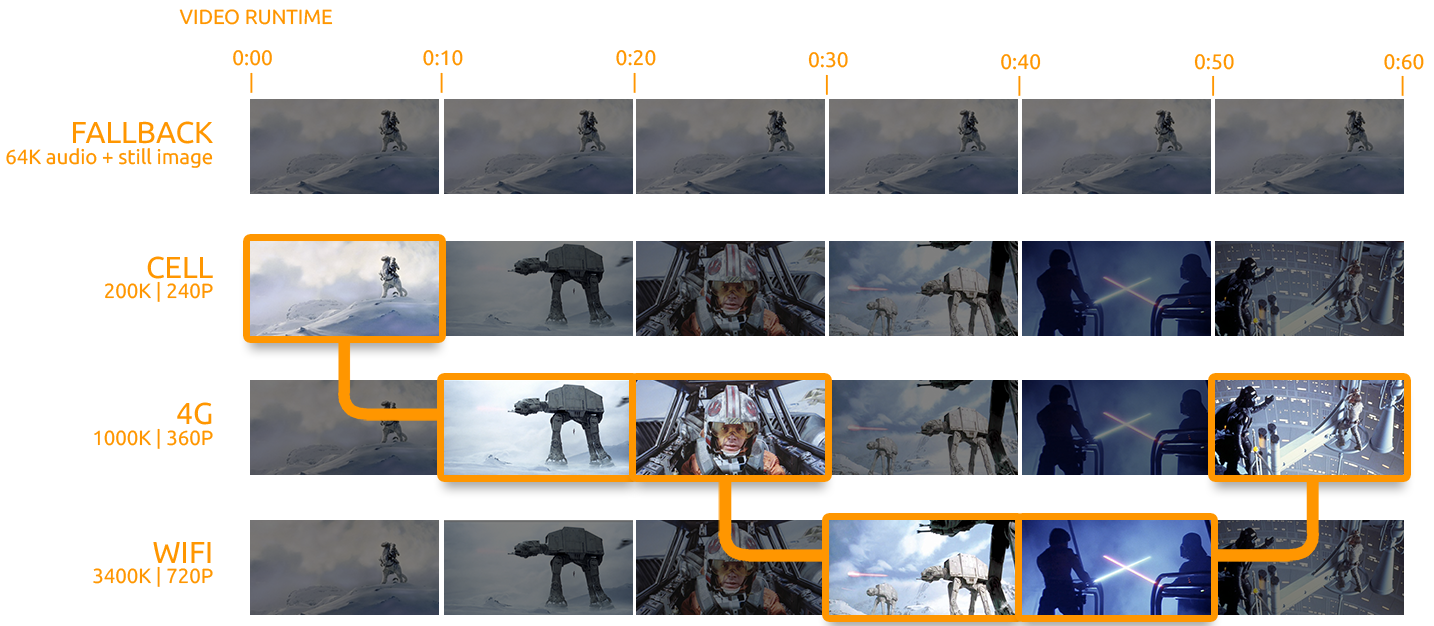
\includegraphics[scale=0.9]{img/timestamp.png}

  El vídeo se codifica en un formato que reproduzcan los clientes.

  Se generan segmentos cortos (10s) de distintas calidades.
\end{frame}

\begin{frame}[fragile]{Archivos de índice}
  Los segmentos de la misma calidad se ordenan en un \textbf{archivo índice}:

\begin{lstlisting}
#EXTM3U
#EXT-X-PLAYLIST-TYPE:VOD
#EXT-X-TARGETDURATION:10
#EXT-X-VERSION:3
#EXT-X-MEDIA-SEQUENCE:0
#EXTINF:10.0,
http://example.com/movie1/fileSequenceA.ts
#EXTINF:10.0,
http://example.com/movie1/fileSequenceB.ts
#EXTINF:10.0,
http://example.com/movie1/fileSequenceC.ts
#EXTINF:9.0,
http://example.com/movie1/fileSequenceD.ts
#EXT-X-ENDLIST
\end{lstlisting}
\end{frame}

\begin{frame}[fragile]{Índice maestro}
  Los archivos índice de las distintas calidades se muestran en uno \textbf{maestro}:
\begin{center}
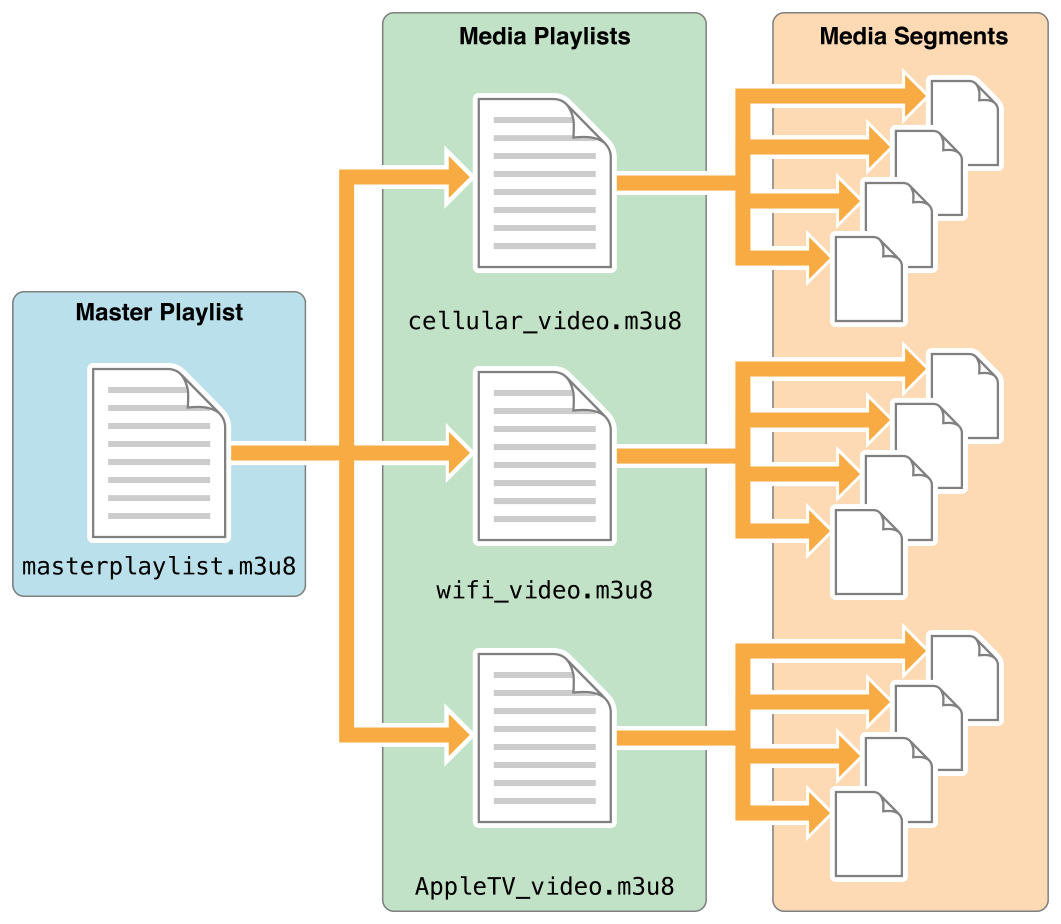
\includegraphics[scale=0.17]{img/indiceMaestro.png}
\end{center}
\end{frame}

\begin{frame}[fragile]{Ejemplo de índice maestro}
\begin{lstlisting}
#EXTM3U
#EXT-X-STREAM-INF:PROGRAM-ID=1, RESOLUTION=720x480
http://ALPHA.mycompany.com/lo/prog_index.m3u8
#EXT-X-STREAM-INF:PROGRAM-ID=1, RESOLUTION=720x480
http://BETA.mycompany.com/lo/prog_index.m3u8

#EXT-X-STREAM-INF:PROGRAM-ID=1, RESOLUTION=1920x1080
http://ALPHA.mycompany.com/md/prog_index.m3u8
#EXT-X-STREAM-INF:PROGRAM-ID=1, RESOLUTION=1920x1080
http://BETA.mycompany.com/md/prog_index.m3u8
\end{lstlisting}
\end{frame}

\begin{frame}[fragile]{Índice en streaming}
\texttt{EXT-X-MEDIA-SEQUENCE} indica el primer segmento disponible:

\begin{lstlisting}
#EXTM3U
#EXT-X-TARGETDURATION:10
#EXT-X-VERSION:3
#EXT-X-MEDIA-SEQUENCE:2
#EXTINF:10,
fileSequence2.ts
#EXTINF:10,
fileSequence3.ts
#EXTINF:10,
fileSequence4.ts
#EXTINF:10,
fileSequence5.ts
\end{lstlisting}
\end{frame}

\begin{frame}[fragile]{Encriptación} %?

\texttt{EXT-X-KEY} indice la clave a utilizar:

\begin{lstlisting}
#EXTM3U
#EXT-X-VERSION:3
#EXT-X-TARGETDURATION:15

#EXT-X-KEY:METHOD=AES-128,URI="https://priv.example.com/key.php?r=52"

#EXTINF:2.833,
http://media.example.com/fileSequence52-A.ts

#EXT-X-KEY:METHOD=AES-128,URI="https://priv.example.com/key.php?r=53"

#EXTINF:15.0,
http://media.example.com/fileSequence53-A.ts
\end{lstlisting}
\end{frame}

\begin{frame}[fragile]{Subtítulos}
Podemos añadir subtítulos en varios idiomas especificando el estilo con CSS:

\begin{lstlisting}
#EXTM3U

#EXT-X-MEDIA:TYPE=CLOSED-CAPTIONS,GROUP-ID="cc",
NAME="CC1",LANGUAGE="en",DEFAULT=YES,AUTOSELECT=YES,INSTREAM-ID="CC1"
#EXT-X-MEDIA:TYPE=CLOSED-CAPTIONS,GROUP-ID="cc",
NAME="CC2",LANGUAGE="sp",AUTOSELECT=YES,INSTREAM-ID="CC2"

#EXT-X-STREAM-INF:BANDWIDTH=1000000,SUBTITLES="subs",CLOSED-CAPTIONS="cc"
x.m3u8
\end{lstlisting}
\end{frame}

\begin{frame}[fragile]{En el cliente (nativo)}
  Basta utilizar el elemento \texttt{video}:

\begin{lstlisting}[language=HTML]
<html>
<head>
    <title>Ejemplo con soporte nativo</title>
</head>
<body>
    <video
        src="http://ejemplo.com/streaming.m3u8"
        height="300" width="400"
        >
    </video>
</body>
</html>
\end{lstlisting}
\end{frame}

\begin{frame}{En el cliente (\texttt{hls.js})}
  \begin{center}
    
\includegraphics[scale=0.2]{img/usohls.png}    
  \end{center}
\end{frame}

\begin{frame}[fragile]{En el cliente (\texttt{hls.js})}
\begin{lstlisting}[language=JavaScript]
var video = document.getElementById('video');
var hls = new Hls();
hls.loadSource('http://ejemplo.com/streaming.m3u8');
hls.attachMedia(video);
hls.on(Hls.Events.MANIFEST_PARSED,function() {
  video.play();
}
\end{lstlisting}
\end{frame}

\end{document}
